\cleardoublepage

\chapter{Introducción}
\label{makereference1}

\begin{quotation}

  El calor aprieta. Tratas de distraerte de las altas temperaturas y aliviar la pesadez del aire con tu programa favorito, refrescante bebida en mano. En cambio, la nevera se mantiene inusualmente silenciosa, el ventilador permanece inmóvil y la televisión no parece despertar. Lentamente, la habitación se sume en la oscuridad.

  Un tiempo después, toda la estancia repentinamente se inunda nuevamente en la luz de las lámparas previamente impotentemente encendidas que vuelven a la vida, el apagón parece haber concluido. Comprendes que, acostumbrado a bastar con apretar el interruptor, rara vez reflexionas en el complejo entramado eléctrico detrás de algo tan simple, que permanece oculto ante la mirada común.

\end{quotation}

El sistema energético tras de la totalidad de la generación, transporte y distribución de la electricidad se mantiene entendiblemente completamente transparente ante los ojos de los usuarios finales de dicha energía~\cite{garrues2009red}.

Por un lado, existe un entramado de redes de transporte eléctrico que combina múltiples tecnologías para asegurar su funcionamiento, teniendo que disponer de una elevada complejidad con el fin de integrar las diversas características del entorno cambiante de los activos energéticos.

Por otro, las partes interesadas realmente compran y venden la energía en masa en el llamado mercado de la electricidad, en el cual se determina finalmente su precio puntual. Esto da lugar a dinámicas de arbitraje con el objetivo de generar beneficio económico, al igual que sucede con cualquier otro activo financiero.

En la actualidad, existen multitud de soluciones energéticas con las que aprovisionar la red de energía y arbitrar en el mercado, como la generación fotovoltaica, eólica, hidráulica o ciclo combinado. Aunque todas ellas juegan un papel más que fundamental en el sistema energético~\cite{turkenburg2000renewable}, una de ellas destaca por encima del resto, especialmente por su creciente popularidad. Se trata de los \glspl{bess}, ilustrados en la figura~\ref{fig:instalacion-bess}.

\begin{figure}
  \centering
  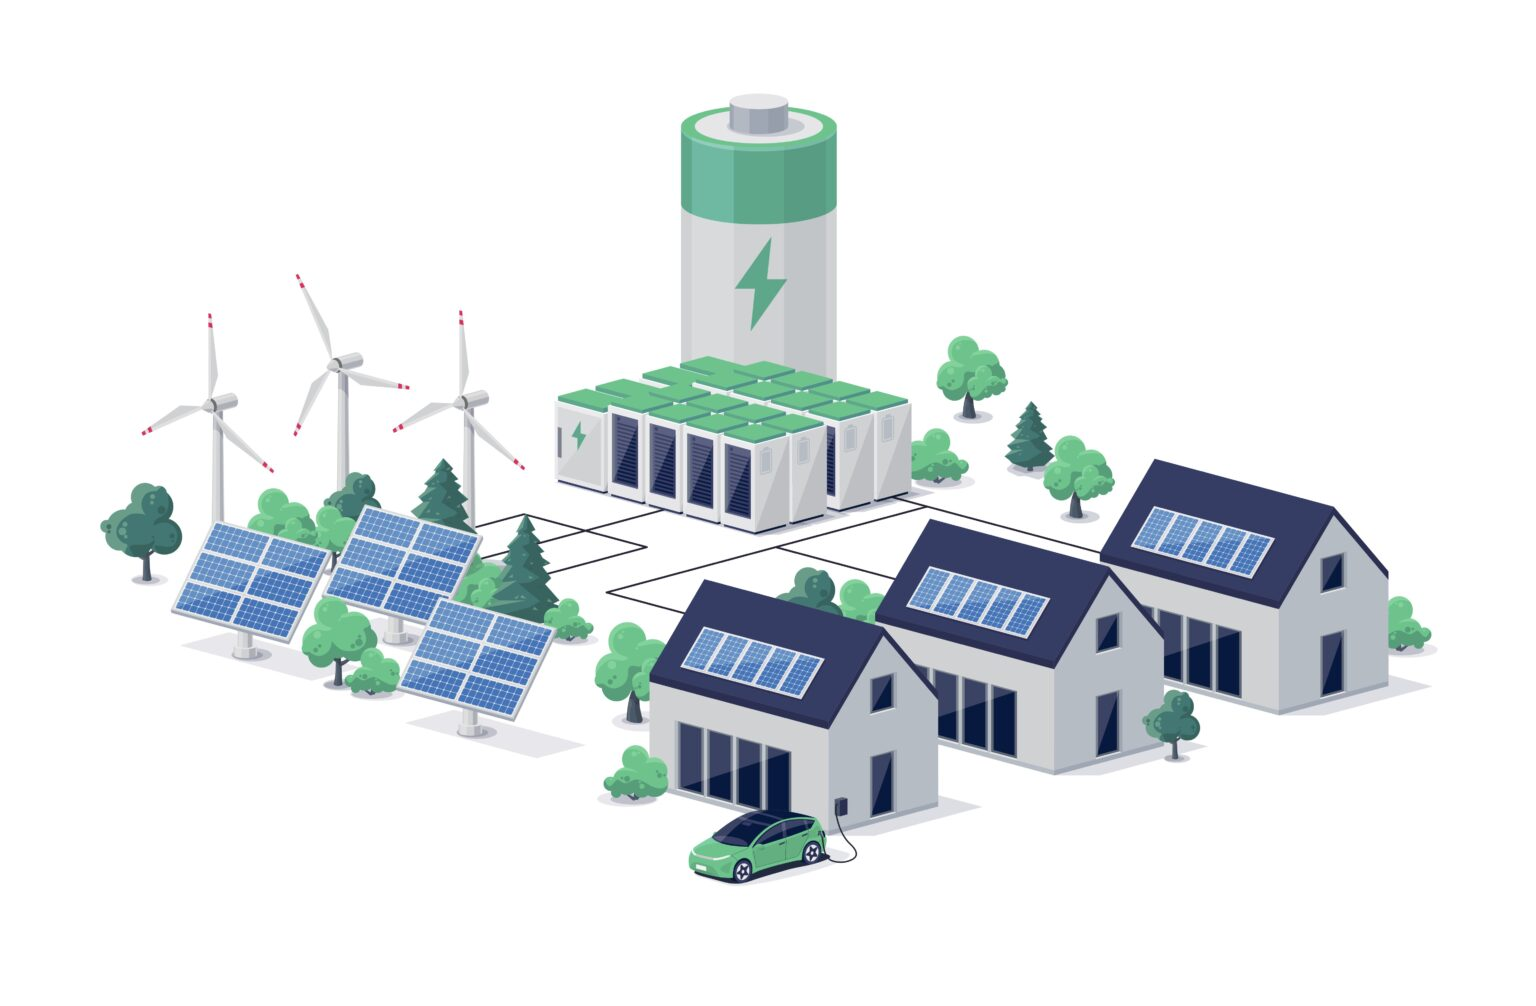
\includegraphics[width=0.5\linewidth]{figures/instalacion-bess.jpg}
  \caption{Ilustración de la disposición una instalación híbrida de generación y almacenamiento~\cite{deutz2023what}.}
  \label{fig:instalacion-bess}
\end{figure}

Precisamente, los \glspl{bess} son una comparativamente novedosa tecnología energética de almacenamiento que permiten, como su propio nombre indica, almacenar electricidad para su uso posterior. Esto facilita enormemente la gestión de la demanda y, crucialmente, mejora la estabilidad y eficiencia de la infraestructura eléctrica, pudiendo regularla activamente gracias a la rápida capacidad de conmutación de las baterías. De esta forma, son una de las tecnologías energéticas más convenientes para evitar posibles desajustes en la red~\cite{xu2014bess}.

Aún y todo, no sirve con disponer únicamente de las baterías, sino que, más que nada, es justamente imprescindible controlar la carga y descarga de estos dispositivos cuidadosamente para prolongar su vida útil y asegurar el correcto funcionamiento de los mismos. Como las baterías cuentan con un \gls{capex} inicialmente considerable, pero un \gls{opex} mínimo~\cite{larsson2018cost}, lo que se busca es su rentabilidad mediante el beneficio generado a través del arbitraje de la energía almacenada en el mercado eléctrico.

Es entonces cuando surge la necesidad de la creación de un sistema de optimización de baterías en el mercado eléctrico basado en el \gls{iiot}, el cual gestione tanto la infraestructura operacional, el entorno de mercado, la modelización estructural y el comando y control, continuamente ciclando la batería indefinidamente en busca de los mejores márgenes. Aún siendo posible realizar parte de dicha gestión manualmente, la complejidad y velocidad de los mercados (teniendo en especial consideración las recientes actualizaciones~\cite{omie2025instruccion}), hacen que la automatización sea altamente relevante.

De hecho, así es como nace \textsc{Optibat}, el sistema de optimización de baterías en el mercado eléctrico de desarrollo propio desplegado satisfactoriamente en múltiples instalaciones energéticas a lo largo del país, que mueve docenas de megavatios hora al día y genera millones de euros de ingresos previstos al año. Consigue solucionar el trabajo de licitación manual de los agentes de mercado a través de la colaboración con los operadores de telecontrol, previamente necesario para la incorporación en el mercado de las posiciones de las baterías.

Con esto, se detallan las decisiones de diseño relacionadas con la integración del sistema y los componentes de la arquitectura ya existentes (es decir, aspectos fundamentales de la operación que la entidad energética dueña de los activos energéticos tiene disponibles con anterioridad), el desarrollo con respecto a la creación de todos los elementos propios a tener en cuenta, la validación para asegurar la seguridad y correcto funcionamiento, el despliegue en relación a la puesta en marcha en instalaciones a gran escala y la experimentación comparativa en busca del mejor modo de operación.

De esta forma, el sistema se divide en los apartados anteriormente mencionados. La infraestructura operacional, explicada en el capítulo~\ref{makereference3}, gestiona la capa de interacción de menor nivel disponible. El entorno de mercado, especificado en el capítulo~\ref{makereference4}, determina la información extraída de las instituciones regulatorias con las que se trabaja. La modelización estructural, puntualizada en el capítulo~\ref{makereference5}, habla de la lógica de negocio de las decisiones a tomar. El comando y control, precisado en el apartado~\ref{makereference6}, explica el flujo de vuelta a los activos físicos y la interacción de los agentes de mercado y operadores de telecontrol con el sistema. Finalmente, se describe la experimentación realizada en el capítulo~\ref{makereference7}.

\section{Objetivos}
\label{makereference1.1}

El objetivo principal es el diseño, desarrollo, validación y despliegue (excluyendo la experimentación) de un sistema de arbitraje de baterías en el mercado eléctrico, garantizando su integración con la infraestructura establecida y su habilitación para operar en el mercado eléctrico. Cabe destacar que, dado que la tecnología de almacenamiento de energía en baterías apenas se encuentra aún en sus primeras etapas de desarrollo, no existe una solución fácilmente integrable o de sencilla implementación sobre la infraestructura energética existente, aunque existan esfuerzos externos para mejorar la situación. Por ello, lo que primeramente se busca es establecer dicha base.

A su vez, se definen varios objetivos secundarios complementarios al objetivo principal anterior, detallados a continuación.

\begin{description}

  \item[Maximizar la rentabilidad] Más allá de hacer funcionar el sistema, obtener la mayor rentabilidad entre la energía comprada y vendida es lo primordial. El sistema debe ser capaz de analizar las previsiones de precios del mercado eléctrico para programar de forma óptima los ciclos de carga y descarga, asegurando la compra de energía en los periodos de menor coste y su venta en los de mayor precio, además de tener en cuanta factores externos al mercado y rentabilizar los \glspl{capex} y \glspl{opex}. Lo más importante es diferenciar el beneficio neto en euros y la rentabilidad en euros por megavatio hora, como determina la \gls{cnmc} en el \gls{boe}~\cite{cnmc2025resolucion}, ya que esta última es la métrica verdaderamente usada para asegurar que se asigna el valor correcto a las unidades de energía usada.

  \item[Minimizar el desgaste de las baterías] Se busca gestionar la operación del activo, principalmente la profundidad de descarga y el número de ciclos, de manera que se prolongue su vida útil y se minimice el desgaste físico del \gls{soc}. Se pretende encontrar el equilibrio entre la rentabilidad a corto plazo y la sostenibilidad de la inversión a largo plazo (ganar mucho dinero cuanto antes pero gastar la batería contra no ofertar tan agresivamente y estabilizar el ciclado pudiendo aprovechar mejores oportunidades futuras). La métrica usada para medir el desgaste se trata del número de ciclos de carga completos que, a diferencia del \gls{soh}, permite estimar la evolución del desgaste más fácilmente.

  \item[Cumplir con los requisitos regulatorios] Es altamente aconsejable que todas las operaciones de carga y descarga propuestas por el sistema se adhieran estrictamente a los requisitos técnicos y normativos impuestos por tanto el \gls{mo} como el \gls{tso}~\cite{crespo2004resolucion}. Esto incluye el respeto de los límites de potencia estructurales marcados por ley, los límites técnicos causados por indisponibilidades, etc. El cumplimiento se mide a través de la magnitud de la desviación final por periodo de mercado en megavatios hora, es decir, la cantidad de energía que el sistema ha pactado pero no ha sido capaz de cubrir.

  \item[Garantizar la seguridad de la operación] Se deben implementar múltiples niveles de validación para prevenir cualquier operación que pueda comprometer la integridad física del \gls{bess} o de la información misma. Aunque el control de bajo nivel es responsabilidad del \gls{bms} nativo de la batería, el sistema de optimización tiene la obligación de operar siempre dentro de un rango seguro predefinido. Además, la información tiene que fluir adecuándose correctamente a la \gls{pera}~\cite{williams1994purdue} de ciberseguridad en el entrono industrial. La seguridad de la operación se mide de forma empírica teniendo en cuenta el número de alarmas causadas por los sistemas de almacenamiento y alertas de ciberseguridad.

  \item[Generalizar el diseño] El diseño de una arquitectura modular y configurable resulta clave para permitir la adaptación del sistema a diferentes instalaciones con capacidades de almacenamiento y configuraciones variadas. El objetivo es crear una solución escalable, no específica a una única instalación, facilitando su despliegue en futuras instalaciones con un esfuerzo de integración mínimo. La modularidad se analiza mediante el número íntegro de instalaciones soportadas por el sistema en el momento de su despliegue.

  \item[Facilitar la monitorización del sistema] Una interfaz de comando y control, que permita a los operadores de telecontrol y agentes de mercado supervisar el estado del sistema en tiempo real, ayuda a aumentar la confianza en el mismo. Esta interfaz debe proporcionar una visualización clara de las operaciones planificadas y ejecutadas y los resultados económicos obtenidos, garantizando la transparencia y la trazabilidad de las decisiones del sistema. Crucialmente, los agentes de mercado deben ser capaces de sobrescribir el comportamiento automático del sistema con indicaciones manuales ante situaciones de mercado no tenidas en cuenta, o periodos de prueba en el caso de los operadores de telecontrol.

  \item[Responder ante fallos] Se dota al sistema de mecanismos de detección y gestión de fallos, tanto internos como, principalmente, externos, para asegurar su robustez y alta disponibilidad. Esto incluye la capacidad de gestionar interrupciones en la operación de la disponibilidad de los activos físicos o la pérdida o información incompleta de los datos de mercado, debiendo tener en cuenta dichas situaciones explícitamente de tal forma que el funcionamiento del sistema, más allá de dicha particularidad, no se vea afectado. Medido programáticamente mediante el número indisponibilidades no causadas por factores externos, sino por el sistema.

  \item[Analizar la viabilidad económica] Utilizando los datos operativos y los resultados del sistema se busca realizar un análisis de viabilidad económica posterior. El objetivo es validar el caso de negocio, cuantificar con precisión la rentabilidad obtenida teniendo en cuenta los \glspl{capex} y \glspl{opex} y modelar el rendimiento financiero del activo bajo diferentes escenarios de mercado. Este análisis sirve para refinar las estrategias de operación y guiar futuras inversiones en los sistemas de almacenamiento de energía en baterías, intentando validar así la aparente predisposición al beneficio de las baterías como activo energético. Se mide en euros megavatio hora relativos. Se trata de un análisis posterior ya que se considera con anterioridad la tesis del beneficio de rentabilidad de los \glspl{bess}.

\end{description}

\section{Alcance}
\label{makereference1.2}

El proyecto se centra exclusivamente en el desarrollo de un sistema de optimización de baterías en el mercado eléctrico integral, de extremo a extremo. Se compone de la infraestructura operacional con la que interactuar con los elementos físicos que forman parte del sistema, la adquisición de la información del entorno de mercado a través de las instituciones regulatorias correspondientes, la modelización estructural de la situación del ciclado de las baterías y de la instalación al completo para la resolución de la optimalidad, y el comando y control para transmitir los resultados de vuelta a la batería y mercado e informar a los agentes de mercado que supervisan los movimientos realizados por el sistema.

En cambio, el alcance no incluye el control físico del nivel eléctrico de las instalaciones, realizado por el \gls{bms} que viene incluido en los \glspl{bess} industriales y es implantado a gran escala por el integrador del sistema, como lo es Ingeteam~\cite{ingeteam2022ingeteam}, debido a obvias consideraciones de seguridad y de acceso físico restringido.

Tampoco se realiza el despliegue en sí del \gls{pis} central, ya que otras tecnologías energéticas hacen uso del mismo más allá de las baterías. Esto no quita que, aunque el sistema de control de planta ya exista de antes, el sistema desarrollado realize la integración de los activos energéticos físicos mismos con el \gls{pis} mismo mediante su extensión, a única excepción de su despliegue.

Finalmente, el proyecto debe considerar procesos externos del entorno en el que es desplegado, por lo que no hay otra opción que depender de la capa de indirección del almacenamiento de la información del entorno de mercado (el \gls{dw}), del desglose de las posiciones negociadas previamente consultadas en servicios internos, y de la última etapa de la realización de las ofertas de mercado, la cual debe, por consideraciones legales, realizarse por la parte confiable de la entidad energética dueña de los activos energéticos.

\section{Plan de trabajo}
\label{makereference1.3}

El plan de trabajo consta de la distribución en tareas del desarrollo del proyecto en su conjunto. Se constituye de la división de los apartados en concordancia con los objetivos, desde el inicio hasta el final del proyecto integrado, y de la explicación de estos.

\begin{figure}[h]
  \centering
  \resizebox{\textwidth}{!}{
    \begin{ganttchart}[link bulge = 1.3, link/.style={-to, rounded corners = 3pt}, milestone/.append style={xscale=5}, time slot format=isodate, time slot unit=day, x unit=1mm]{2025-02-10}{2025-09-15}
      \gantttitlecalendar{month=shortname}\\
      \ganttgroup[name=analisis]{Análisis preliminar}{2025-02-10}{2025-03-05}\\
      \ganttbar[name=normativa]{Estudio de la normativa}{2025-02-10}{2025-02-16}\\
      \ganttbar[name=mercado]{Formación en el mercado eléctrico}{2025-02-17}{2025-02-23}\\
      \ganttbar[name=baterias]{Formación en baterías}{2025-02-24}{2025-03-05}\\
      \ganttbar[name=herramientas]{Evaluación de las herramientas}{2025-02-17}{2025-03-05}\\
      \ganttgroup[name=desarrollo]{Desarrollo}{2025-03-10}{2025-07-31}\\
      \ganttbar[name=diseño]{Diseño del optimizador}{2025-03-10}{2025-04-06}\\
      \ganttbar[name=cuartohorario]{Adaptación a mercados cuartohorarios}{2025-03-10}{2025-03-23}\\
      \ganttmilestone[name=aislado]{Topología aislada}{2025-04-07}\\
      \ganttbar[name=generacion]{Colocación renovable}{2025-04-08}{2025-05-29}\\
      \ganttmilestone[name=hibrido]{Topología híbrida}{2025-05-30}\\
      \ganttbar[name=conector]{Incorporación del sistema de información de planta}{2025-04-08}{2025-05-15}\\
      \ganttbar[name=señales]{Pruebas unitarias de señalización}{2025-05-16}{2025-05-29}\\
      \ganttbar[name=entorno]{Consideración parcial del entorno de mercado}{2025-05-16}{2025-05-29}\\
      \ganttmilestone[name=pruebas]{Despliegue en preproducción}{2025-06-03}\\
      \ganttbar[name=control]{Consignación y licitaciones}{2025-06-04}{2025-06-30}\\
      \ganttbar[name=mo]{Obtención de datos del operador de mercado}{2025-06-04}{2025-06-13}\\
      \ganttbar[name=tso]{Obtención de datos del operador del sistema}{2025-06-14}{2025-06-26}\\
      \ganttmilestone[name=produccion]{Despliegue en producción}{2025-07-01}\\
      \ganttbar[name=mandos]{Cuadro de mando}{2025-06-14}{2025-07-17}\\
      \ganttbar[name=incidencias]{Resolución de incidencias}{2025-06-04}{2025-07-31}\\
      \ganttgroup[name=experimentacion]{Experimentación}{2025-07-01}{2025-08-17}\\
      \ganttbar[name=rendimiento]{Pruebas de integración de rendimiento}{2025-07-01}{2025-07-31}\\
      \ganttbar[name=comparaciones]{Análisis comparativos locales}{2025-08-01}{2025-08-17}\\
      \ganttgroup[name=redaccion]{Redacción del informe}{2025-07-01}{2025-09-15}\\
      \ganttbar[name=estructuracion]{Estructuración de los apartados}{2025-07-01}{2025-7-21}\\
      \ganttbar[name=typesetting]{Composición tipográfica}{2025-07-15}{2025-8-31}\\
      \ganttbar[name=contenido]{Elaboración del contenido}{2025-07-15}{2025-8-31}\\
      \ganttbar[name=revision]{Revisión y edición}{2025-08-25}{2025-9-15}\\
      \ganttlink{normativa}{mercado}
      \ganttlink{mercado}{baterias}
      \ganttlink[link type=s-s]{typesetting}{contenido}
      \ganttlink[link type=s-s]{diseño}{cuartohorario}
      \ganttlink{diseño}{aislado}
      \ganttlink{aislado}{generacion}
      \ganttlink{generacion}{hibrido}
      \ganttlink{conector}{señales}
      \ganttlink{hibrido}{pruebas}
      \ganttlink{señales}{pruebas}
      \ganttlink{entorno}{pruebas}
      \ganttlink{pruebas}{control}
      \ganttlink{mo}{tso}
      \ganttlink{tso}{produccion}
      \ganttlink{control}{produccion}
      \ganttlink{rendimiento}{comparaciones}
    \end{ganttchart}
  }
  \caption{Diagrama Gantt del plan de trabajo.}
  \label{fig:plan-trabajo}
\end{figure}

% TODO
\begin{description}

  \item[Estudio de la normativa] Investigación de la regulación del mercado eléctrico.

  \item[Formación en el mercado eléctrico] Formación sobre el funcionamiento y los procesos del mercado eléctrico.

  \item[Formación en baterías] Estudio de las características técnicas de los \gls{bess}.

  \item[Evaluación de las herramientas] Análisis de las herramientas existentes y elección de las tecnologías.

  \item[Diseño del optimizador] Diseño de la arquitectura de la optimización exclusivamente centrada en el comportamiento de las baterías.

  \item[Adaptación a mercados cuartohorarios] Adaptación del sistema para su operación en los nuevos mercados cuartohorarios, diario, intradiarios y continuo.

  \item[Topología aislada] Habilitación de la optimización para topologías aisladas.

  \item[Colocación renovable] Desarrollo de la lógica para gestionar baterías junto a una planta de generación renovable colocadas.

  \item[Topología híbrida] Habilitación de la optimización para topologías híbridas.

  \item[Incorporación del sistema de información de planta] Despliegue y configuración de las conexiones con los activos energéticos del \gls{pis}.

  \item[Pruebas unitarias de señalización] Verificación independiente de la correcta comunicación de lectura y señalización de consignas del \gls{pis}.

  \item[Consideración parcial del entorno de mercado] Realización de la primera integración parcial con datos de mercado no programáticos.

  \item[Despliegue en preproducción] Instalación del sistema en un entorno de pruebas sin acceso a licitaciones en el mercado.

  \item[Consignación y licitaciones] Desarrollo de la capacidad de enviar órdenes a las baterías y ofertas al mercado.

  \item[Obtención de datos del operador de mercado] Automatización de la obtención de información relevante publicada por el \gls{mo}.

  \item[Obtención de datos del operador del sistema] Implementación de la recepción de datos técnicos y de red del \gls{tso}.

  \item[Despliegue en producción] Puesta en marcha del sistema en instalaciones reales para su operación comercial.

  \item[Cuadro de mando] Creación del cuadro de mandos para la monitorización y el control del sistema.

  \item[Resolución de incidencias] Corrección continua de los errores y problemas que surgen durante la operación del sistema.

  \item[Pruebas de integración de rendimiento] Medición del rendimiento global (en terminos monetarios) con todos sus componentes.

  \item[Análisis comparativos locales] Evaluación y comparación de diferentes estrategias de operación.

  \item[Estructuración de los apartados] Organización del contenido y definición de la estructura del informe final del proyecto.

  \item[Composición tipográfica] Maquetación y formateo del documento.

  \item[Elaboración del contenido] Redacción del cuerpo principal del informe describiendo todo el trabajo realizado.

  \item[Revisión y edición] Realización de la corrección final del documento para pulir el texto y eliminar errores.

\end{description}
